% Revised sleep-protocol subsection (2026-10-08). Replaces the previous
% \subsection{Sleep-protocol} and its tikz schematic. Labels sec:sp_SG,
% eq:decay, eq:wakeup and fig:weight_dynamics are kept so existing
% cross-references still resolve. Needs \usepackage{booktabs} for the table.
% Figure: figures/sleep_trace_BW.pdf, built by src/plot_sleep_trace.py from
% results/sleep_trace/ (one MNIST batch, seed 42, r = 0.3).

\subsection{Sleep protocol}\label{sec:sp_SG}

We interleave training with offline sleep episodes on a fixed schedule. Training time is divided into intervals of $I = 3500$ simulation steps, corresponding to $35$ images at $100$ steps each, and at the first step of every interval the simulator enters a \emph{hard-pause} sleep episode of
\begin{equation}
T_{\mathrm{sleep}} = \max\!\left(1, \left\lfloor r \cdot I \right\rceil\right)
\label{eq:tsleep}
\end{equation}
iterations, where $r$ is the \textit{sleep ratio}. The episode runs in virtual time: the real simulation clock does not advance and no images are consumed, so every sleep ratio sees the same images in the same order and differs only in how much offline processing is inserted between them. The ratio is therefore defined relative to wake time rather than to total time; at $r = 0.3$, the value used in the comparisons with conventional regularization and in the ablation, each episode lasts $1050$ iterations and sleep accounts for $r/(1+r) \approx 23\%$ of all iterations.

Each sleep iteration combines four operations, which the ablation switches on and off separately. First, sensory input is suppressed by setting all input spikes to zero. Second, the membrane potential of every neuron receives additive Gaussian noise $\xi \sim \mathcal{N}(0, \sigma^2)$ with $\sigma^2 = 2$, which is absent during wake and drives spontaneous spiking in the absence of input. Third, every nonzero synapse is pulled toward a target magnitude by the power-law operator
\begin{equation}
|w_i(k+1)| = w_{\mathrm{tgt}} \left(\frac{|w_i(k)|}{w_{\mathrm{tgt}}}\right)^{\lambda}, \qquad 0 < \lambda < 1,
\label{eq:decay}
\end{equation}
where $k$ indexes sleep iterations, $w_{\mathrm{tgt}} = 0.5$ for both excitatory and inhibitory synapses, and the sign of inhibitory weights is restored after the update. Fourth, the same STDP rule that operates during wake is applied to the spontaneous spikes, after which weights are clipped to their admissible range as on every wake step. Eq.~\eqref{eq:decay} is not a decay in the usual sense: weights above $w_{\mathrm{tgt}}$ shrink while weights below it grow, and because $x \mapsto x^{\lambda}$ is monotone, the operator preserves the rank order of the weights within each group.

\subsubsection{Log-space form and calibration of the sleep rate}

The power law becomes linear under a logarithmic change of variables. Defining the log-gap of each synapse as $u_i = \ln\!\left(|w_i| / w_{\mathrm{tgt}}\right)$, Eq.~\eqref{eq:decay} reduces to $u_i(k+1) = \lambda\, u_i(k)$, so that after $n$ iterations
\begin{equation}
u_i(k+n) = \lambda^{n}\, u_i(k).
\label{eq:logspace}
\end{equation}
Consequently, $n$ iterations at rate $\lambda$ are exactly equivalent to a single application of Eq.~\eqref{eq:decay} with exponent $\lambda^{n}$, and the fraction of every log-gap that survives an episode, $s = \lambda^{T_{\mathrm{sleep}}}$, is the same for every synapse regardless of its current weight. Inverting Eq.~\eqref{eq:logspace} gives the number of iterations required for any prescribed contraction, $n = \ln s / \ln \lambda$, or, for a prescribed duration, the rate that achieves it, $\lambda = s^{1/n}$.

We use the second relation to decouple sleep duration from the strength of the homeostatic pull. With a fixed $\lambda$, the contraction per episode $\lambda^{T_{\mathrm{sleep}}}$ would shrink geometrically with the sleep ratio, so that a sweep over $r$ would confound the time spent asleep with the amount of downscaling. We instead hold the contraction per batch of $1000$ training images fixed at $\rho = 0.4$ and derive the rate from the sleep ratio,
\begin{equation}
\lambda(r) = \rho^{\,1 / \left(E \, T_{\mathrm{sleep}}(r)\right)}, \qquad E = \left\lfloor \frac{1000 \cdot 100 - 1}{I} \right\rfloor = 28,
\label{eq:lambda_r}
\end{equation}
where $E$ is the number of sleep episodes per batch. Every episode then retains the fraction $s = \rho^{1/E} \approx 0.968$ of each log-gap, closing $3.2\%$ of the distance to $w_{\mathrm{tgt}}$ in log space irrespective of $r$ (Table~\ref{tab:lambda_r}). Sleep conditions therefore differ only in how many noise-driven iterations, with STDP active, the same downscaling is spread across.

\begin{table}[h!]
\centering
\caption{Sleep duration and power-law rate for representative sleep ratios, from Eqs.~\eqref{eq:tsleep} and \eqref{eq:lambda_r} with $I = 3500$, $E = 28$, and $\rho = 0.4$. The contraction per episode, $s = \lambda^{T_{\mathrm{sleep}}}$, is identical for all ratios.}
\label{tab:lambda_r}
\begin{tabular}{rrcc}
\toprule
$r$ & $T_{\mathrm{sleep}}$ & $\lambda(r)$ & $s = \lambda^{T_{\mathrm{sleep}}}$ \\
\midrule
$0.1$ & $350$  & $0.9999065$ & $0.968$ \\
$0.3$ & $1050$ & $0.9999688$ & $0.968$ \\
$0.5$ & $1750$ & $0.9999813$ & $0.968$ \\
$1.0$ & $3500$ & $0.9999907$ & $0.968$ \\
\bottomrule
\end{tabular}
\end{table}

\subsubsection{Episode termination}

Every episode runs for its full $T_{\mathrm{sleep}}$ iterations. Before each iteration the implementation also checks whether the total synaptic weight of both groups, $\mathcal{W}_x = \sum_i |w_i|$ over the nonzero synapses of group $x \in \{E, I\}$, lies within $0.1\%$ of its value at the start of training,
\begin{equation}
\left|\mathcal{W}_x(k) - \mathcal{W}_x(0)\right| \leq 10^{-3}\, \mathcal{W}_x(0) \quad \text{for both } x \in \{E, I\},
\label{eq:wakeup}
\end{equation}
and ends the episode early if so. Wake STDP has already raised $\mathcal{W}_E$ to $1.6\%$ above $\mathcal{W}_E(0)$ when the first episode begins and keeps raising it thereafter (Fig.~\ref{fig:weight_dynamics}a), and because Eq.~\eqref{eq:decay} pulls individual weights toward $w_{\mathrm{tgt}}$ rather than steering the sum toward $\mathcal{W}_x(0)$, the condition was not met in any of the $28$ episodes of the traced run. In practice, sleep duration is set by $T_{\mathrm{sleep}}$ alone, and the contraction per episode is exactly $s$.

\begin{figure}[h!]
\centering
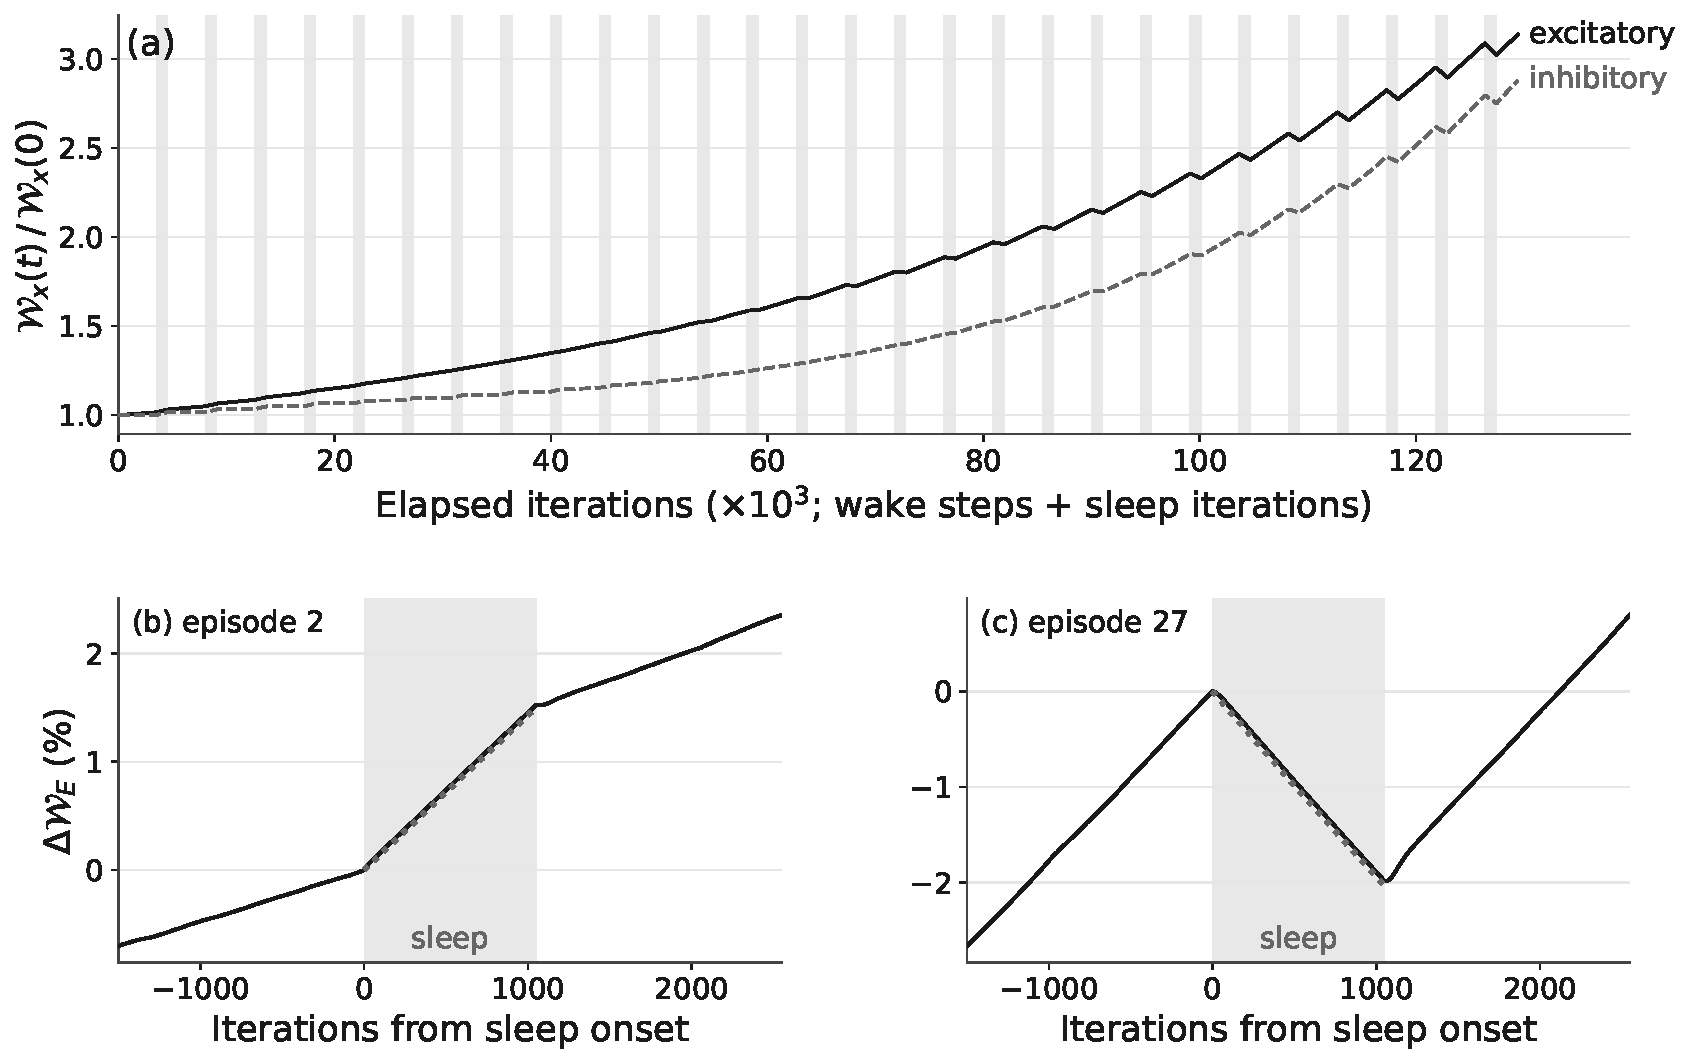
\includegraphics[width=\linewidth]{figures/sleep_trace_BW.pdf}
\caption{Weight dynamics across the wake--sleep cycle in one training batch on MNIST ($r = 0.3$, seed 42). \textbf{(a)} Total excitatory (solid) and inhibitory (dashed) weight relative to its initial value, against elapsed iterations (wake steps plus virtual sleep iterations); grey bands mark the $28$ sleep episodes of $1050$ iterations each. \textbf{(b, c)} Change in total excitatory weight around an early and a late episode. The dotted line is the trajectory predicted by the power-law operator alone (Eq.~\eqref{eq:logspace}), computed from the weights at sleep onset. Early in training most weights lie below $w_{\mathrm{tgt}}$ and sleep raises the total weight (b); once the mean weight reaches $w_{\mathrm{tgt}}$, sleep lowers it (c).}
\label{fig:weight_dynamics}
\end{figure}

Figure~\ref{fig:weight_dynamics} shows the resulting weight dynamics in a training run on MNIST at $r = 0.3$. Over one batch, wake STDP increases the total excitatory and inhibitory weight roughly threefold, whereas each sleep episode changes the total by at most $2\%$. The direction of that change follows from Eq.~\eqref{eq:decay}: early in training most weights lie below $w_{\mathrm{tgt}}$ and sleep raises the total weight (Fig.~\ref{fig:weight_dynamics}b), and from the $14$th episode onward, when the mean excitatory weight reaches $w_{\mathrm{tgt}}$, sleep lowers it (Fig.~\ref{fig:weight_dynamics}c). Within every episode the recorded trajectory lies within $0.1\%$ of the trajectory predicted by the power law alone, and the measured contraction of the log-gaps, $\mathrm{sd}(u_{\mathrm{after}}) / \mathrm{sd}(u_{\mathrm{before}})$, ranges from $0.968$ to $0.972$ across the $28$ episodes against the calibrated $s = 0.968$. Noise-driven STDP thus contributes little to the weight change during sleep at this operating point.

Taken together, the entire process from initial input to recurrent processing, and finally, sleep, is described in Algorithm~\ref{alg:train}.
